\documentclass[12pt,a4paper,onecolumn]{article}
\usepackage[utf8]{inputenc}
\usepackage[T1]{fontenc}
\usepackage[french]{babel}

% ------------------------- Color table ----------------------------------------
\usepackage{multirow}
\usepackage[table]{xcolor}
\definecolor{maroon}{cmyk}{0,0.87,0.68,0.32}
% ------------------------------------------------------------------------------

\usepackage{amscd}
\usepackage{amsthm}
\usepackage{physics}
\usepackage[left=2.2cm,right=2.2cm,top=2cm,bottom=2cm]{geometry}
\usepackage{textcomp,gensymb} %pour le °C, et textcomp pour éviter les warning
\usepackage{graphicx} %pour les images
\usepackage{caption}
\usepackage{subcaption}
\usepackage[colorlinks=true,
	breaklinks=true,
	citecolor=blue,
	linkcolor=blue,
	urlcolor=blue]{hyperref} % pour insérer des liens
\usepackage{epstopdf} %converting to PDF
\usepackage[export]{adjustbox} %for large figures

\usepackage{array}
\usepackage{dsfont}% indicatrice : \mathds{1}


% -------------------------- Mathematics ---------------------------------------
\graphicspath{{images/}} % For the images path
% ------------------------------------------------------------------------------

% -------------------------- Mathematics ---------------------------------------
\usepackage{mathrsfs, amsmath, amsfonts, amssymb}
\usepackage{bm}
\usepackage{mathtools}
\usepackage[Symbol]{upgreek} % For pi \uppi different from /pi
\newcommand{\R}{\mathbb{R}} % For Real space
% ------------------------------------------------------------------------------


% -------------------------- Code format ---------------------------------------
\usepackage[numbered,framed]{matlab-prettifier}
\lstset{
	style              = Matlab-editor,
	basicstyle         = \mlttfamily,
	escapechar         = '',
	mlshowsectionrules = true,
}
% ------------------------------------------------------------------------------

% ------------------------- Blbiographie --------------------------------------
% \usepackage[backend=biber, style=science]{biblatex}
% \addbibresource{biblio.bib}
% ------------------------------------------------------------------------------


\setcounter{tocdepth}{4} %Count paragraph
\setcounter{secnumdepth}{4} %Count paragraph
\usepackage{float}

\usepackage{graphicx} % for graphicspath
% \graphicspath{{../images/}}

\usepackage{array,tabularx}
\newcolumntype{L}[1]{>{\raggedright\let\newline\\\arraybackslash\hspace{0pt}}m{#1}}
\newcolumntype{C}[1]{>{\centering\let\newline\\\arraybackslash\hspace{0pt}}m{#1}}
\newcolumntype{R}[1]{>{\raggedleft\let\newline\\\arraybackslash\hspace{0pt}}m{#1}}

\newcommand{\assignmenttitle}{}
\newcommand{\studentname}{}
\newcommand{\email}{}
\newcommand{\schoolyear}{2017/2018}


\title{
\normalfont \normalsize 
\textsc{Object recognition and computer vision, Master MVA, \schoolyear} \\
[10pt] 
\rule{\linewidth}{0.5pt} \\[6pt] 
\huge \assignmenttitle \\
\rule{\linewidth}{2pt}  \\[10pt]
}

\author{\studentname}

\date{\small\email}

\newcommand{\question}[1]{\subsubsection*{#1}}

\setlist[enumerate]{topsep=0pt,itemsep=-1ex,partopsep=1ex,parsep=1ex,label=(\roman*)}

\graphicspath{{images/}}

\newcommand{\labelnotempty}[1]{
\def\temp{#1}\ifx\temp\empty
\else
    \label{#1}
\fi
}
% single figure
\newcommand{\singlefig}[4]{
\begin{figure}[ht!]
        \centering
        \includegraphics[width={#2}\columnwidth]{#1}
        \caption{#3}
        \labelnotempty{#4}
\end{figure}}

\newcommand{\subfig}[4]{
\includegraphics[width={#2}\columnwidth]{#1}
\caption{#3}
\labelnotempty{#4}
}

% double figure
\newcommand{\doublefig}[4]{
\begin{figure}[ht!]
    \centering
    \begin{subfigure}[t]{0.45\columnwidth}
        \centering
    #1
    \end{subfigure}
    ~
    \begin{subfigure}[t]{0.45\columnwidth}
        \centering
    #2
    \end{subfigure}
    \caption{#3}
    \labelnotempty{#4}
\end{figure}}

% triple figure
\newcommand{\triplefig}[5]{
\begin{figure}[ht!]
    \centering
    \begin{subfigure}[t]{0.30\columnwidth}
        \centering
    #1
    \end{subfigure}
    ~
    \begin{subfigure}[t]{0.30\columnwidth}
        \centering
    #2
    \end{subfigure}
    ~
    \begin{subfigure}[t]{0.30\columnwidth}
        \centering
    #3
    \end{subfigure}
    \caption{#4}
    \labelnotempty{#5}
\end{figure}}



% ------------------------ General informations --------------------------------
\title{Sub_pixel_image_processing_tp_5}
\author{Vincent Matthys}
\graphicspath{{images/}}
% ------------------------------------------------------------------------------


\begin{document}

\begin{tabularx}{0.9\textwidth}{@{} l X r @{} }
	{\textsc{Master MVA}}               &  & \textsc{TP5}       \\
	\textsc{Sub-pixel image processing} &  & {ENS Paris Saclay} \\
\end{tabularx}
\vspace{1.5cm}
\begin{center}

	\rule[11pt]{5cm}{0.5pt}

	\textbf{\LARGE \textsc{Compte-rendu TP5}}
	\vspace{0.5cm}

	Vincent Matthys

	vincent.matthys@ens-paris-saclay.fr

	\rule{5cm}{0.5pt}

	\vspace{1.5cm}
\end{center}
%
\section{Exerice 13}
\setcounter{subsection}{1}
\subsection{Zoom d'un facteur 2 d'un signal discret}

Appelant \(\tilde{u}\) l'interpolée linéaire de \(v\), \(\forall n \in \mathbb{Z}\) :
\begin{equation}
	\begin{split}
		v[2n] &=  \tilde{u}(\frac{2n}{2}) = u[n]\\
		v[2n + 1] &= \tilde{u}(\frac{2n + 1}{2}) = \frac{u[n] + u[n + 1]}{2}\\
	\end{split}
\end{equation}

On peut donc exprimer la transformée de Fourier de \(v\) suivant :

\begin{equation}
	\begin{split}
		\hat{v}(\xi) &= \sum_{k\in\mathbb{Z}}v[k]e^{-ik\xi} \quad \forall \xi \in \mathbb{R}\\
		\hat{v}(\xi) &= \sum_{\substack{k = 2n \\n\in\mathbb{Z}}}v[2n]e^{-i2n\xi} + \sum_{\substack{k = 2n + 1 \\n\in\mathbb{Z}}}v[2n + 1]e^{-i(2n+1)\xi}\\
		\hat{v}(\xi) &= \sum_{\substack{k = 2n \\n\in\mathbb{Z}}}u[n]e^{-in(2\xi)} + \sum_{\substack{k = 2n + 1 \\n\in\mathbb{Z}}}\frac{u[n] + u[n + 1]}{2}e^{-i(2n+1)\xi}\\
		\hat{v}(\xi) &= \hat{u}(2\xi) + \sum_{n\in\mathbb{Z}}\frac{u[n]}{2}e^{-i(2n+1)\xi} + \sum_{n\in\mathbb{Z}}\frac{u[n + 1]}{2}e^{-i(2n+1)\xi}\\
		\hat{v}(\xi) &= \hat{u}(2\xi) + \frac{e^{-i\xi}}{2}\sum_{n\in\mathbb{Z}}\frac{u[n]}{2}e^{-in(2\xi)} ++ \frac{e^{i\xi}}{2}\sum_{n\in\mathbb{Z}}\frac{u[n + 1]}{2}e^{-i(n + 1)(2\xi)}\\
		\hat{v}(\xi) &= \hat{u}(2\xi)\left(1 + \cos\left(\xi\right)\right)
	\end{split}
	\label{zoom_lin}
\end{equation}

D'autre part, l'interpolée \(U\) de Shannon de \(v\), par le théorème de Shannon, s'exprime comme :

\begin{equation}
	\begin{split}
		U(x) &= \sum_{k\in\mathbb{Z}} u[k]sinc(x-k) \quad \forall x \in \mathbb{R}\\
	\end{split}
	\label{th_shannon}
\end{equation}

S'ensuit une première opération de zoom par 2, représentée par le signal \(W\) :
\begin{equation}
	\begin{split}
		W(x) &= U(\frac{x}{2}) \quad \forall x \in \mathbb{R}\\
	\end{split}
\end{equation}

Dont la transformée de Fourier s'exprime :

\begin{equation}
	\begin{split}
		\hat{W}(\xi) &= \int_{\mathbb{R}}U(\frac{x}{2})e^{-ix\xi}dx \quad \forall \xi \in \mathbb{R}\\
		&= \int_{\mathbb{R}}U(x)e^{-ix(2\xi)}dx\\
		&= \hat{U}(2\xi)\\
		&=  \int_{\mathbb{R}}\sum_{k\in\mathbb{Z}} u[k]sinc(x-k) e^{-ix(2\xi)} \quad \text{d'après \eqref{th_shannon}}\\
		&= \sum_{k\in\mathbb{Z}} u[k] e^{-ik(2\xi)}\int_{\mathbb{R}} sinc(x-k) e^{-i(x-k)(2\xi)}dx\\
		&= \sum_{k\in\mathbb{Z}} u[k] e^{-ik(2\xi)} \mathds{1}_{[-\pi, \pi]}(2\xi)\\
		&= \hat{u}(2\xi)\mathds{1}_{[-\pi, \pi]}(2\xi)\\
	\end{split}
\end{equation}

On peut alors discrétiser pour obtenir \(\hat{w}\), zoom d'un facteur 2 par interpolée de Shannon :

\begin{equation}
	\left\{
	\begin{split}
		\hat{w}(\xi) &= \hat{u}(2\xi) \quad \forall \xi \in [-\frac{\pi}{2}, \frac{\pi}{2}]\\
		\hat{w}(\xi) &= 0 \quad \forall \xi \in [-\pi, \pi] \setminus [-\frac{\pi}{2}, \frac{\pi}{2}]\\
		\hat{w}(\xi) &: 2\pi-\text{periodisée}
	\end{split}
	\right.
	\label{zoom_shannon}
\end{equation}

Ce qui correspond à un zoom par 0-padding. Ce qui est bien différent du zoom par interpolée linéaire, obtenu en~\eqref{zoom_lin}, où la transformée de Fourier est modulée par un facteur \(1 + \cos(\xi)\).

\subsection{Zoom d'un facteur 2 d'une image discrète}

\textit{Non réussi}

% Appelant \(\tilde{u}\) l'interpolée bilinéaire de \(v\), \(\forall (k,l) \in \mathbb{Z}^2\) :
% \begin{equation}
% 	\begin{split}
% 		v[2k,2l] &=  \tilde{u}\left(\frac{2k}{2}, \frac{2l}{2}\right) = u[k, l]\\
% 		v[2k + 1, 2l] &=  \tilde{u}\left(\frac{2k + 1}{2}, \frac{2l}{2}\right) = \frac{u[k + 1, l] + u[k, l]}{2}\\
% 		v[2k, 2l + 1] &=  \tilde{u}\left(\frac{2k}{2}, \frac{2l + 1}{2}\right) = \frac{u[k, l] + u[k, l + 1]}{2}\\
% 		v[2k + 1, 2l + 1] &=  \tilde{u}\left(\frac{2k + 1}{2}, \frac{2l}{2}\right) = \frac{u[k + 1, l] + u[k, l]}{2}\\
% 	\end{split}
% \end{equation}

\setcounter{section}{16}
\section{Exerice 17}

Pour l'image \textit{crop\_bouc.pgm}, on constate que tous les zoom par interpolation autre que plus proche voisins donne des phénomènes de repliement de spectre, avec notamment une inversion à 90 degrés des tuyaux le long des bords de l'image aggrandie, comme on peut le constater en bas de l'image en figure~\ref{fig_bouc_3}. Ceci est valable quelque soit l'ordre de l'interpolation utilisée. A l'inverse, même si le résultat est moins plaisant à l'oeil, on ne constate pas ce défaut en figure~\ref{fig_bouc_nn}, que nous qualifierons donc de meilleure, car ne présentant pas ce défaut.

\begin{figure}[H]
	\centering
	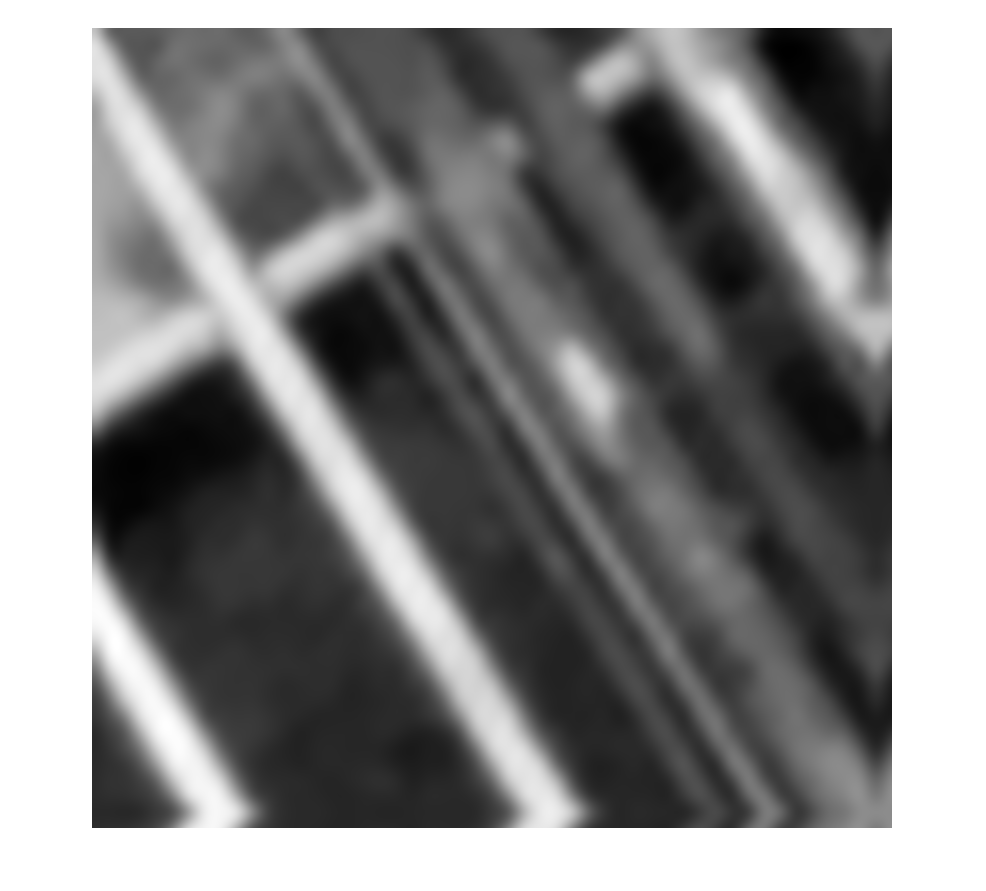
\includegraphics[height = 0.4\textheight]{bouc_3}
	\caption{Zoom par interpolée de spline 3 de l'image bouc}
	\label{fig_bouc_3}
\end{figure}

\begin{figure}[H]
	\centering
	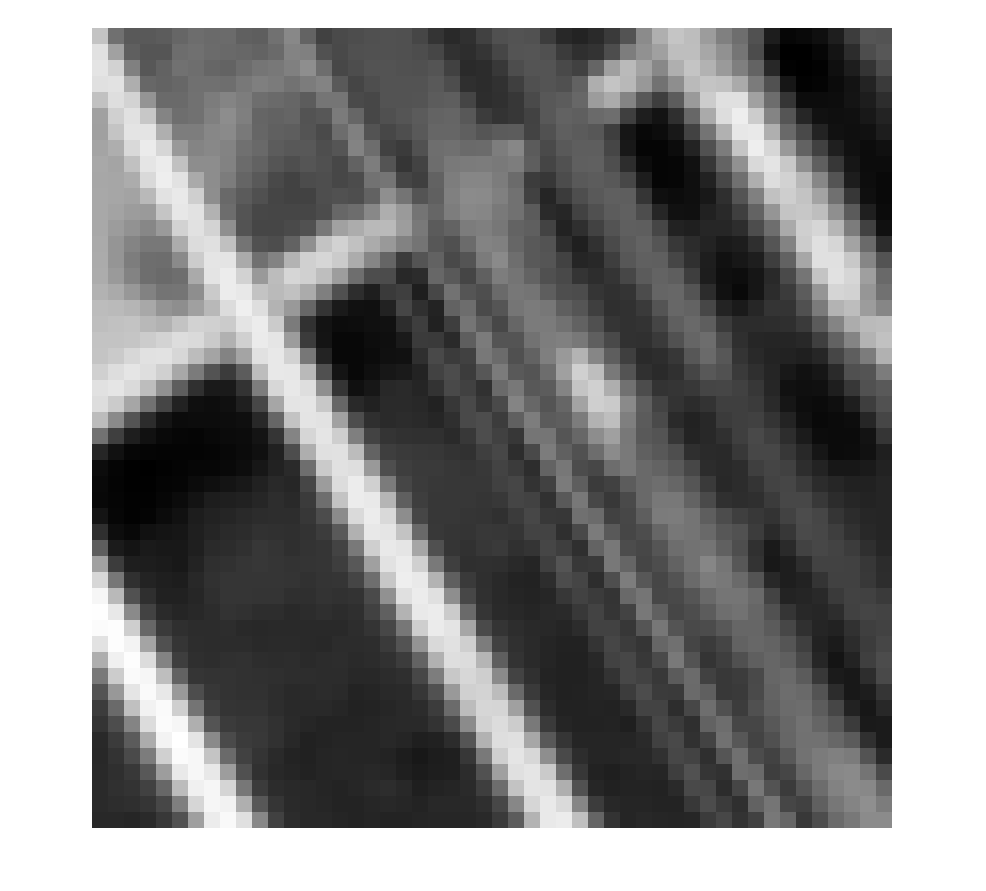
\includegraphics[height = 0.4\textheight]{bouc_nn}
	\caption{Zoom par interpolée des plus proches voisins de l'image bouc}
	\label{fig_bouc_nn}
\end{figure}

En figure~\refeq{fig_bouc_ff} est visualisé le module de la transformée de Fourier de l'image cameraman en entier. On peut constater le phénomène d'alias présent et observé, provenant de la deuxième croix oblique, lorsqu'on sur-échantillonne ce spectre. Les conditions du théorème de Shannon n'étant plus vérifiées l'image est aliasée.
\begin{figure}[H]
	\centering
	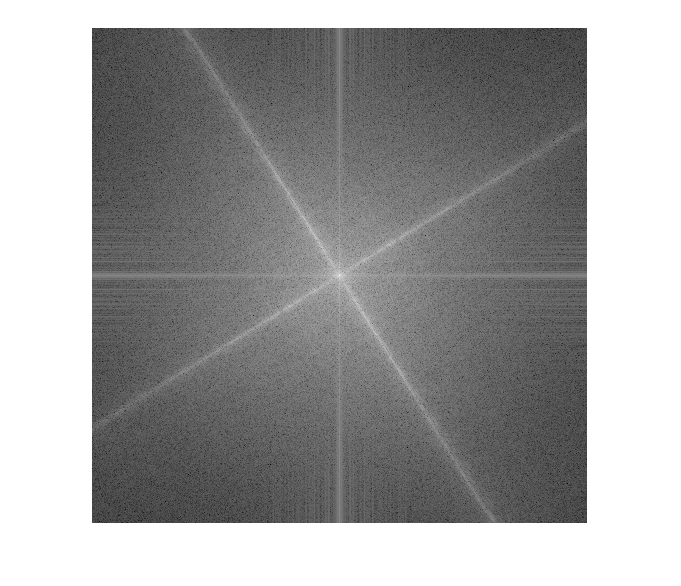
\includegraphics[height = 0.4\textheight]{bouc_ff}
	\caption{Transformée de Fourier du bouc entier}
	\label{fig_bouc_ff}
\end{figure}


Pour l'image \textit{crop\_cameran.pgm}, on ne constate aucun effet notable de repliement de spectre lors du zoom, et ce pour toutes les méthodes d'interpolation. On préférera alors une interpolée d'ordre maximale . Ceci est valable quelque soit l'ordre de l'interpolation utilisée. En revanche, on constate un défaut de ringing d'autant plus important que l'ordre d'interpolation est grande. On préferera donc prendre une interpolée spline d'ordre 3, dont le zoom résultant est présenté en figure~\ref{fig_cam_3}, faible, présentant le meilleur compromis entre le phénomène de ringing et le respect de la géométrie de l'image. On peut même envisager de prendre le résultat de l'interpolée linéaire, présenté en figure~\ref{fig_cam_lin}, d'odre encore inférieure, limitant ce phénomène. Le prix à payer étant le non recolllement des dérivées des lignes de niveau de l'image.

\begin{figure}[H]
	\centering
	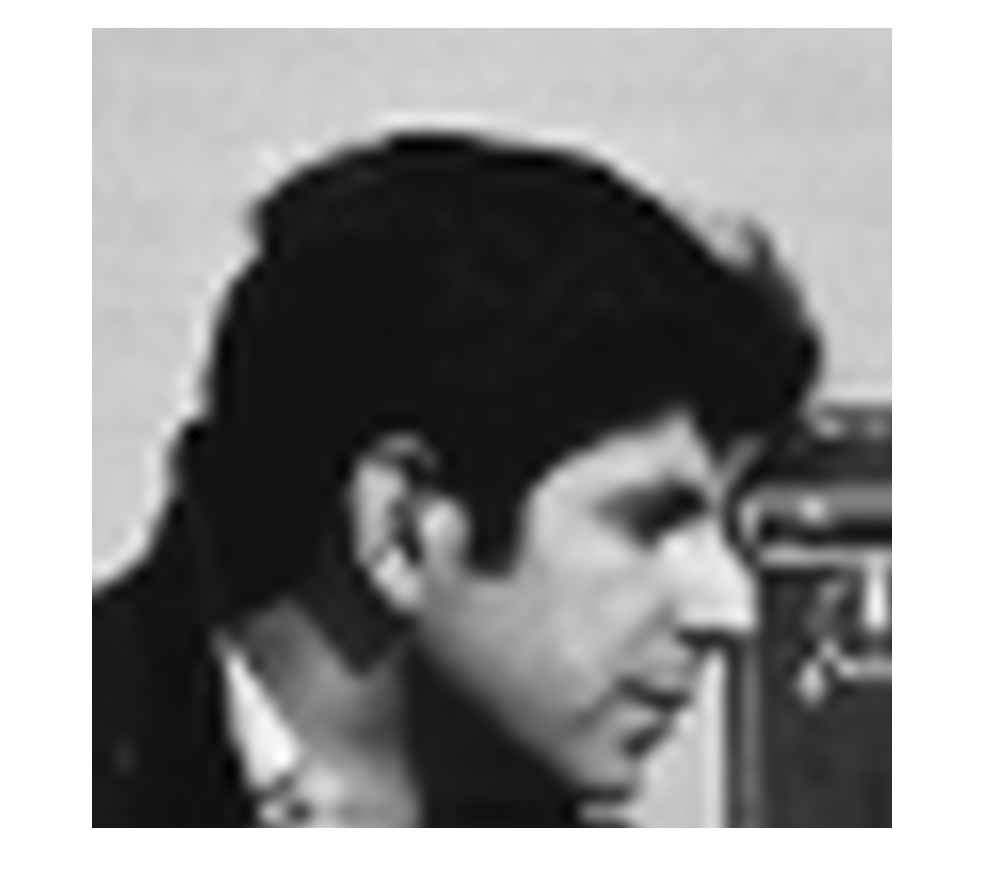
\includegraphics[height = 0.4\textheight]{cam_3}
	\caption{Zoom par interpolée spline d'ordre 3 de l'image cameraman}
	\label{fig_cam_3}
\end{figure}

\begin{figure}[H]
	\centering
	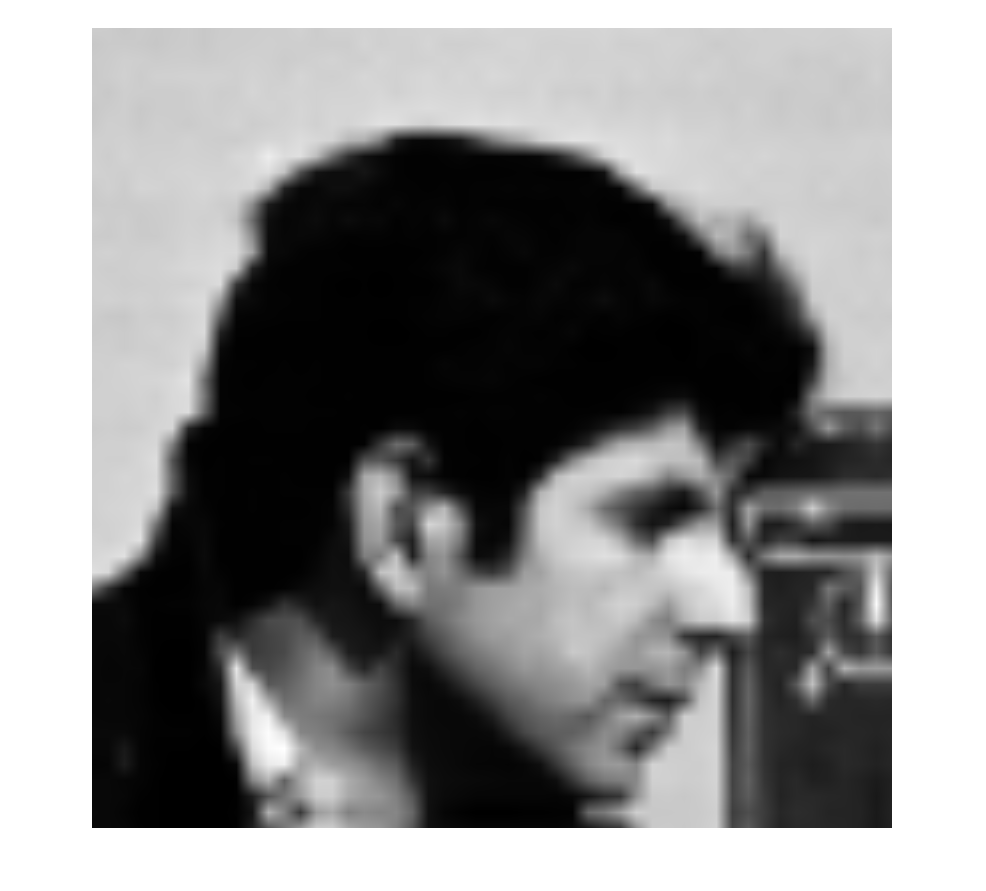
\includegraphics[height = 0.4\textheight]{cam_lin}
	\caption{Zoom par interpolée linéaire de l'image cameraman}
	\label{fig_cam_lin}
\end{figure}

En figure~\refeq{fig_ff_cam} est visualisé le module de la transformée de Fourier de l'image cameraman en entier. On constate, contraitement au spectre de bouc, que l'intensité décroit assez vite avec la distance au centre, limitant les phénomène d'aliasing lors du sur-échantillonnage.
\begin{figure}[H]
	\centering
	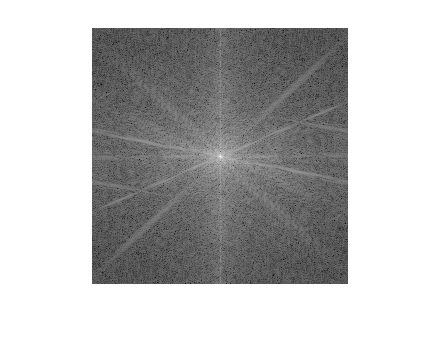
\includegraphics[height = 0.4\textheight]{cam_ff}
	\caption{Transformée de Fourier du cameraman entier}
	\label{fig_ff_cam}
\end{figure}



\end{document}
